\documentclass[../../main.tex]{subfiles}
\begin{document}
\textbf{Notes :} On présente ici les bases fondamentales. L'idée n'est pas (pour l'instant) de faire un cours d'architecture des processeurs (à voir pour un autre cours de Minitel). C'est d'ailleurs très incomplet. Certains détails sont ajoutés durant la partie sur le langage C. Ces détails vont probablement être déplacés ici dans un futur plus ou moins proche. À voir.
\section{Architecture matérielle}
\subsection{Vue de haut} \label{sub:vue_de_haut}
On peut considérer un ordinateur comme un système évoluant selon des entrées pour produire des sorties :
\begin{center}
  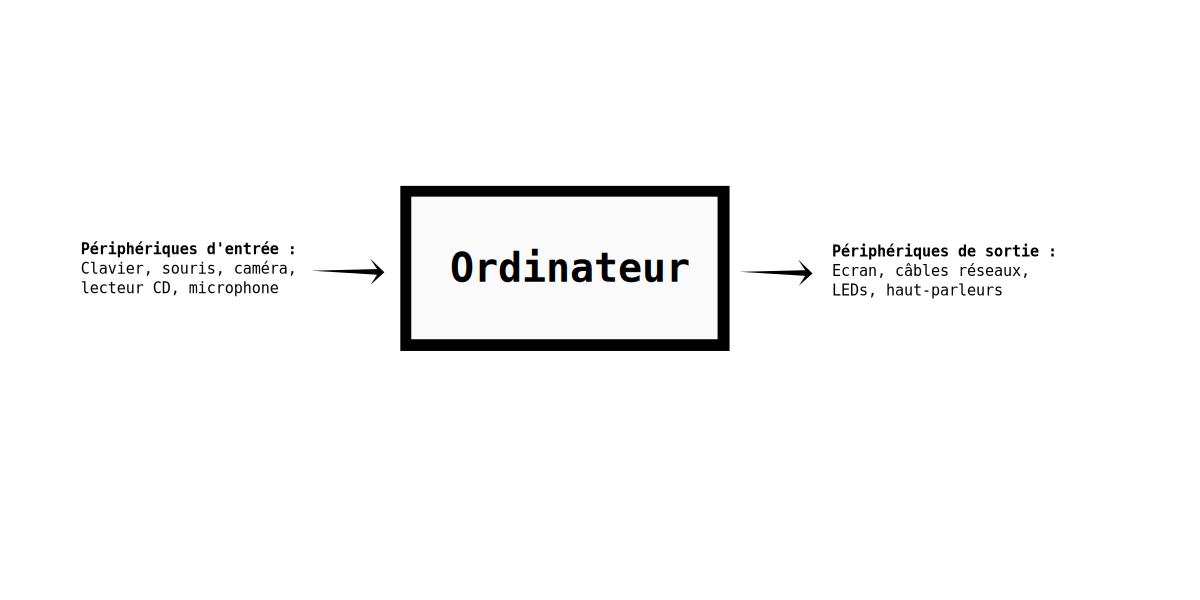
\includegraphics[width=\textwidth]{system}
\end{center}
Ces entrées et sorties sont captés et produites via des appareils appelés périphériques d'entrée/sortie. On garde généralement l'acronyme \textit{E/S} (\textit{\underline{E}ntrée/\underline{S}ortie})\footnote{\textit{\underline{I}nput/\underline{O}utput} en anglais}.

\begin{minitelbasicbox}{\textbf{Petit apparté :} De la rigueur de la définition d'un ``ordinateur''}
Un ordinateur est appareil qui ``calcule''. La signification mathématique du terme ``calculer'' n'a
rien d'évidente. Calculer est au départ une notion que l'on peut qualifier d'assez intuitive et il
est donc difficile d'apporter une définition formelle claire qui satisfasse ce qu'un humain peut
subjectivement appeler le ``calcul''.

Le calcul est le plus généralement associé à une série d'actions pouvant être automatisés par un système physique. Certains modèles théoriques représentent cette automatisation et sont d'ailleurs constructibles (comme le modèle RAM qui se rapproche beaucoup des ordinateurs classiques). Il existe en fait des modèles mathématiques parfaitement abstraits dont on a montré qu'ils sont absolument équivalents aux modèles plus ``intuitifs'' d'ordinateurs.

Ce qui résulte principalement des analyses de ces modèles de calcul est que certains problèmes ne peuvent pas être résolus par des ordinateurs, quelles que soient la forme de ceux-ci, tant qu'ils fonctionnent par le calcul\footnote{C'est-à-dire : même en supposant qu'ils aient une puissance et une vitesse de calcul arbitrairement grande et une mémoire infinie.}.
\end{minitelbasicbox}
L'acronyme \textit{E/S} est extrêmement récurrent puisqu'il apparaît dans tous les cas où existe un système d'entrée et de sortie d'informations.
\subsection{À l'intérieur}
\label{sub:_l_int_rieur}
Les périphériques E/S permettent l'interaction avec le système de l'ordinateur. Pourtant, celui-ci peut très bien fonctionner sans. Par exemple, on lisait les résultats des premiers ordinateurs directement à l'intérieur, et on y entrait les programmes ``à la main'', en modifiant les branchements des câbles pour ``écrire le programme''. En soi, cette notion d'écriture est assez récente, puisqu'elle date des ordinateurs disposant d'un clavier et d'un écran, périphériques E/S fondamentaux pour une interaction ``facile'' avec un ordinateur.

L'ordinateur lui-même est uniquement un calculateur possédant une mémoire. Il est représenté de manière par le schéma ci-dessous qui représente la modélisation d'un ordinateur selon l'\textit{architecture de Von Neumann\footnote{Mathématicien et physicien, John von Neumann a travaillé sur ce modèle et a publié en 1945 un rapport sur la conception de l'ordinateur EDVAC. Ce modèle est donc vieux et présente des limitations comme cela va être souligné.}} :
\begin{center}
  \includesvg[height=6cm]{structure_von_neumann}
  \captionof{figure}{Architecture de Von Neumann \label{fig:von_neumann}}
\end{center}
\textbf{Remarque :} En considérant seulement le système du processeur, la mémoire peut aussi être vue comme un support d'entrée/sortie. Ainsi, la lecture d'une information dans la mémoire constitue une entrée du processeur, et l'écriture d'une information dans la mémoire constitue une sortie du processeur.

\subsubsection{Unité Centrale de Calcul}
\label{ssub:unit_centrale_de_calcul}
L'\textbf{UAL} (\underline{U}nité \underline{A}rithmétique et \underline{L}ogique) est constituée de circuits électroniques qui permettent d'effectuer toutes les opérations fondamentales de calcul, comme l'addition, la multiplication, la soustraction, la ou la division.

L'\textbf{UCP} (\underline{U}nité de \underline{C}ontrôle de \underline{P}rogramme) supervise l'UAL, et contrôle son exécution. Elle s'occupe en particulier de ``comprendre'' les instructions lues dans la mémoire pour faire exécuter par l'UAL les opérations correctes. Elle effectue aussi le passage d'une instruction à l'autre.

L'UCP et l'UAL forment l'\textbf{UCC} (\underline{U}nité \underline{C}entrale de \underline{C}alcul, \textbf{CPU} en anglais), ou plus simplement \textit{processeur}. Si l'UCP et l'UAL sont assemblés en un seul circuit, on parle alors de \textit{microprocesseur}.

\definition{Instruction}{Une instruction est une séquence d'octets qui peut être lue par l'UCC pour exécuter une action.}

\subsubsection{Mémoire}
\label{ssub:m_moire}
La mémoire elle-même n'est dans les faits pas constituée d'un unique bloc mais de plusieurs supports de mémoire dont la vitesse et la capacité varient. On distingue par ordre de vitesse croissante et de capacité décroissante :
\begin{itemize}
    \item les bandes magnétiques (très lents, capacité native de $18\ To$ avec la technologie LTO-9, voir \url{https://fr.wikipedia.org/wiki/Linear_Tape-Open})
    \item les disques durs (lents, capacité allant de $250\ Go$ à $2\ To$)
    \item la mémoire RAM (pour \underline{R}andom \underline{A}ccess \underline{M}emory) (rapide, capacité allant de $1\ Go$ à $8\ Go$, et par agrégation jusqu'à $128\ Go$ voire plus).
    \item la mémoire SRAM  (pour \underline{S}tatic RAM) (5 à 10 fois plus rapide que la RAM, même capacité mais beaucoup plus chère)
    \item les registres (extrêmement rapide, capacité allant de 1 octet à 8 octets, 16 octets pour les ordinateurs spécialisés en calcul scientifique), forment un système de stockage de capacité très (très (très)) faible, destiné à stocker des valeurs temporaires. Ils servent en particulier de tampons pour les calculs du processeur.
\end{itemize}
\begin{center}
\begin{tabular}{|l|l|l|l|}
\hline
\textbf{Type} & \textbf{Temps d'accès} & \textbf{Débit} & \textbf{Capacité} \\
\hline
Disques durs & $3 - 20\ \rm{ms}$ & $10 - 320\ \rm{Mio/s}$ & de l'ordre du $\rm{Tio}$ \\
Mémoire RAM & $5 - 60\ \rm{ns}$ & $1 - 20\ \rm{Gio/s}$ & de l'ordre du $\rm{Gio}$ \\
Mémoire SRAM & $2 - 3\ \rm{ns}$ & & de l'ordre du $\rm{Mio}$ \\
Registres & $\leq 1\ \rm{ns}$ & & de l'ordre du $\rm{Kio}$ \\
\hline
\end{tabular}
\captionof{table}{Caractéristiques des différents supports mémoires \label{tab:carac_mem}}
\end{center}

\subsection{Limitation du modèle de Von Neumann}
\label{sub:limitation_du_mod_le_de_von_neumann}
Le modèle de calcul présenté ci-dessus impose des échanges extrêmement réguliers entre le processeur et la mémoire. Cependant, l'accès à la mémoire est beaucoup plus lent que la vitesse à laquelle les calculs sont effectués par le processeur. En effet, la plupart des processeurs modernes effectuent une opération élémentaire de calcul en un quart de nanoseconde, ce qui est d'au moins un ordre de grandeur plus rapide que l'accès à la mémoire RAM (voir table \ref{tab:carac_mem}).

Pour cette raison, les constructeurs de processeurs ont situé les registres directement dans le (micro-)processeur pour minimiser les temps d'accès et ont ajouté une mémoire supplémentaire au sein du processeur appelée \textit{mémoire cache}, plus rapide que la mémoire RAM, qui est chargée avec les données de la RAM souvent utilisées. L'idée est que le temps d'accès ultérieur à ces données souvent utilisées sera plus court. Un processeur peut posséder plusieurs niveaux de mémoire cache, notés\footnote{``L'' pour \textit{\underline{L}evel}} $L_1, L_2, \dots$. Chaque niveau est plus lent que le précédent mais a une capacité plus élevé. Plus une donnée est utilisée souvent et localement, plus bas sera le niveau de cache utilisé et plus rapide sera donc l'accès. 

La structure de donnée utilisée pour la mémoire cache est une table d'association, ou dictionnaire (voir la section \ref{sec:dictionnaires}).

Finalement, on peut donner un schéma (un peu) plus précis d'un ordinateur moderne : 
\begin{center}
  \includesvg[height=8cm]{structure_moderne}
  \captionof{figure}{Architecture moderne\label{fig:proc_moderne}}
\end{center}
\section{Architecture logicielle}
\label{sec:architecture_logicielle}
Pas encore écrit\dots juste quelques définitions.
\definition{BIOS}{Le BIOS (\textit{\underline{B}asic \underline{I}nput \underline{O}utput \underline{S}ystem}) est le programme qui s'exécute au démarrage de l'ordinateur (appelé le \textit{boot}). C'est lui qui permet de le lancer véritablement pour être utilisé. En effet, son objectif est de ``passer la main'' au système d'exploitation, grâce à un petit programme appelé le \textit{bootloader} (\textit{loader} signifie chargeur en anglais).

\begin{minipage}{\textwidth}
  \begin{center}
    \small
    \includesvg[width=1\textwidth]{bios}
  \end{center}
\end{minipage}
}

\definition{Système d'exploitation}{Un système d'exploitation est un programme exécuté par le BIOS juste après le lancement. Ce programme fournie à l'utilisateur de l'ordinateur toutes les fonctionnalités dont il pourrait avoir besoin : accès au disque dur, accès à la mémoire vive, aux périphériques entrée/sortie, possibilité d'exécuter des programmes utilisateurs, générateur de nombres pseudo-aléatoire, etc\dots

\begin{minipage}{\textwidth}
  \begin{center}
    \includesvg[width=.7\textwidth]{niveau_abstraction}
  \end{center}
\end{minipage}
}
\definition{Fichier}{Un fichier est un ensemble d'informations numériques constituées d'une séquence d'octets. Ces informations peuvent représenter des données allant du programme informatique à la vidéo en passant par les informations d'une communication réseaux, un livre numérique, la mémoire d'un programme informatique, etc\dots Ces informations sont réunis sous un même nom et manipulé comme une unité, appelé le fichier. Les métadonnées d'un fichier fournissent des informations externes complémentaires.

\begin{minipage}{\textwidth}
  \begin{center}
    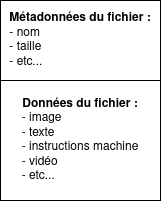
\includegraphics[width=.25\textwidth]{fichier}
  \end{center}
\end{minipage} 
}

\definition{Extension de nom fichier}{Une extension de nom de fichier (ou plus simplement ``extension de fichier'') est une suite de caractères à la fin du nom du fichier, séparée du radical du nom de fichier par un point, qui indique à l'utilisateur de l'ordinateur et aux logiciels le format des données qu'il contient. L'extension agit uniquement à titre \textit{indicatif} ! La modifier sans modifier le fichier lui-même n'effectue STRICTEMENT AUCUNE conversion. Il ne suffit pas d'appeler un chat un chien pour que celui-ci se transforme subitement ! Le nom d'un fichier est seulement une étiquette. Il n'a aucune incidence sur ce que le fichier contient réellement.\footnote{J'insiste car il s'agit là d'une \textit{croyance} extrêmement répandue chez les utilisateurs non techniciens d'outils informatiques}}

\definition{Répertoire et système de fichiers}{Un répertoire est le nom technique donné au dossier. Il s'agit simplement d'un conteneur d'autres répertoires ou fichiers. Il permet de \textit{répertorier} des fichiers ou d'autres répertoires. Sa fonction principale est donc la classification. Afin de faciliter la localisation et la gestion des répertoires et des fichiers, ceux-ci sont organisés suivant un \textit{système de fichiers}. C'est ce système qui permet à l'utilisateur de répartir les fichiers dans une arborescence de répertoires et de les localiser par un chemin d'accès.
\begin{center}
\begin{forest}
[Documents
  [repertoire\_parent
    [repertoire\_enfant\_1
      [fichier\_texte]
      [fichier\_image]
    ]
    [repertoire\_enfant\_2
      [fichier\_video]
    ]
  ]
]
\end{forest}
\end{center}
}

\definition{Répertoire de travail}{Le répertoire de travail d'un exécutable est le répertoire dans lequel l'exécutable va effectuer ses instructions. Par exemple, si l'exécutable contient une instruction qui ouvre et lit un fichier sur le disque dur, l'ordinateur essaiera d'ouvrir ce fichier dans le répertoire de travail, renverra une erreur si ce fichier n'est pas présent dans le répertoire de travail. Il est possible de modifier le répertoire de travail d'un exécutable à l'intérieur de celui-ci (par certaines instructions).}

\definition{Chemin d'accès}{Chaîne de caractères qui décrit la position du fichier sur son support de stockage au sein du système de fichiers. On distingue deux types de chemin d'accès : 
\begin{itemize}
     \item chemin absolu : décrit la position absolue du fichier depuis la racine de l'arborescence du système de fichiers ($/$ sous Linux, $C:/$ sous Windows)
     \item chemin relatif : décrit la position relative du fichier par rapport au répertoire de travail. On considère alors le répertoire de travail comme la racine de l'arborescence
\end{itemize}
\begin{center}
\begin{forest}
[racine
  [...]
  [home
    [user
      [repertoire\_1
        [fichier\_1]
      ]
      [repertoire\_2
        [fichier\_2]
      ]
    ]
  ]
  [...]
]
\end{forest}
\end{center}
Ci-dessus, le chemin absolu du fichier 1 est \textit{racine/home/user/repertoire\_1/fichier\_1}. Si on suppose que le répertoire de travail est \textit{racine/home/user/repertoire\_1}, alors le chemin relatif du fichier 2 est \textit{../repertoire\_2/fichier\_2}.

En effet, ``.'' désigne le nom du répertoire de travail, et ``..'' désigne le répertoire parent du répertoire de travail. Ainsi, \textit{../repertoire\_2} désigne le chemin relatif depuis le répertoire 1 équivalent au chemin absolu \textit{racine/home/user/}
}

\end{document}
